\section{基本概念}
\subsection{三大学派}
人工智能研究的三大学派:
\begin{figure}[htbp]
    \centering
    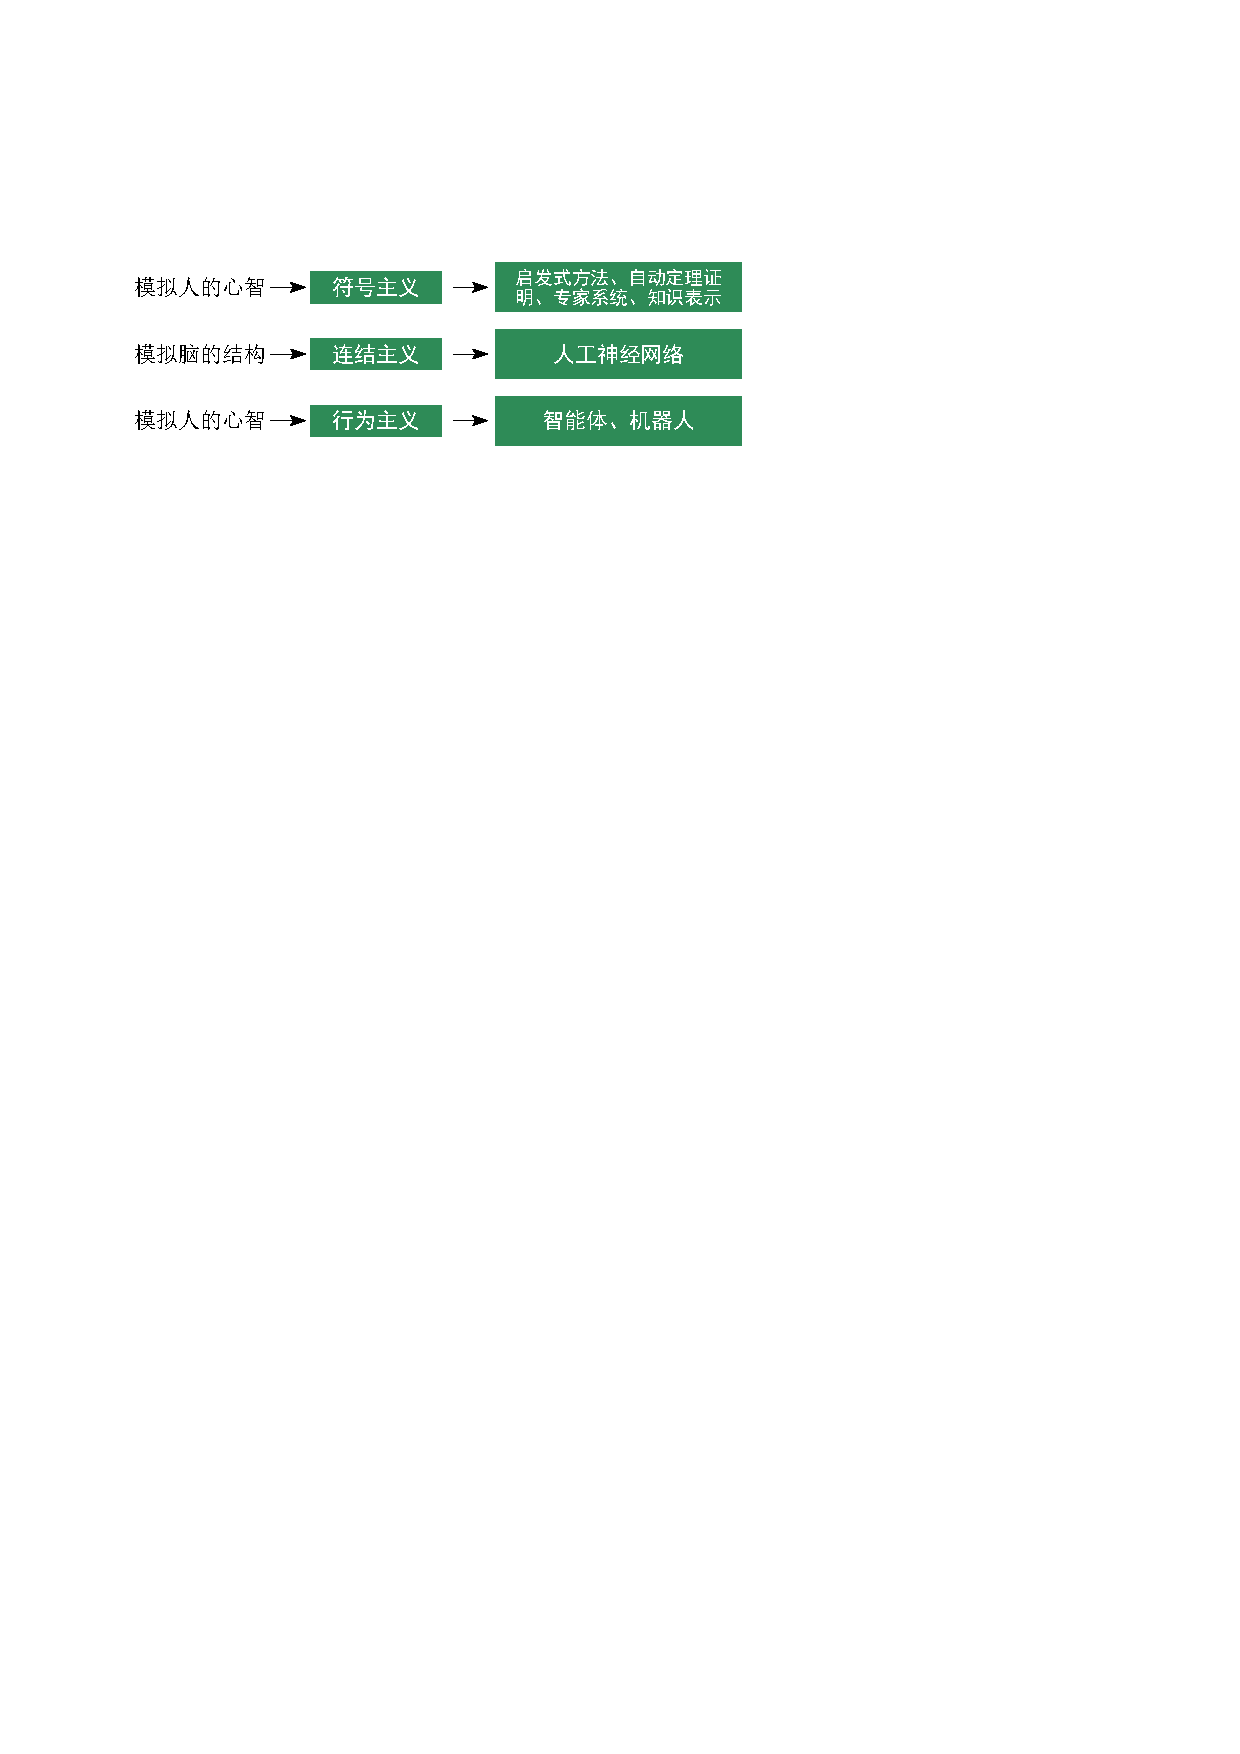
\includegraphics{image/3大学派.pdf}
\end{figure}
\begin{itemize}
    \item 符号主义学派的核心是符号演算与机器推理
    \item 连接主义学派的核心是神经网络与深度学习
    \item 行为主义学派推崇控制、自适应与进化计算
\end{itemize}

\subsection{Agent}
Agent是能够通过传感器感知环境,并且通过执行器对环境产生影响的任何东西。
\begin{figure}[htbp]
    \centering
    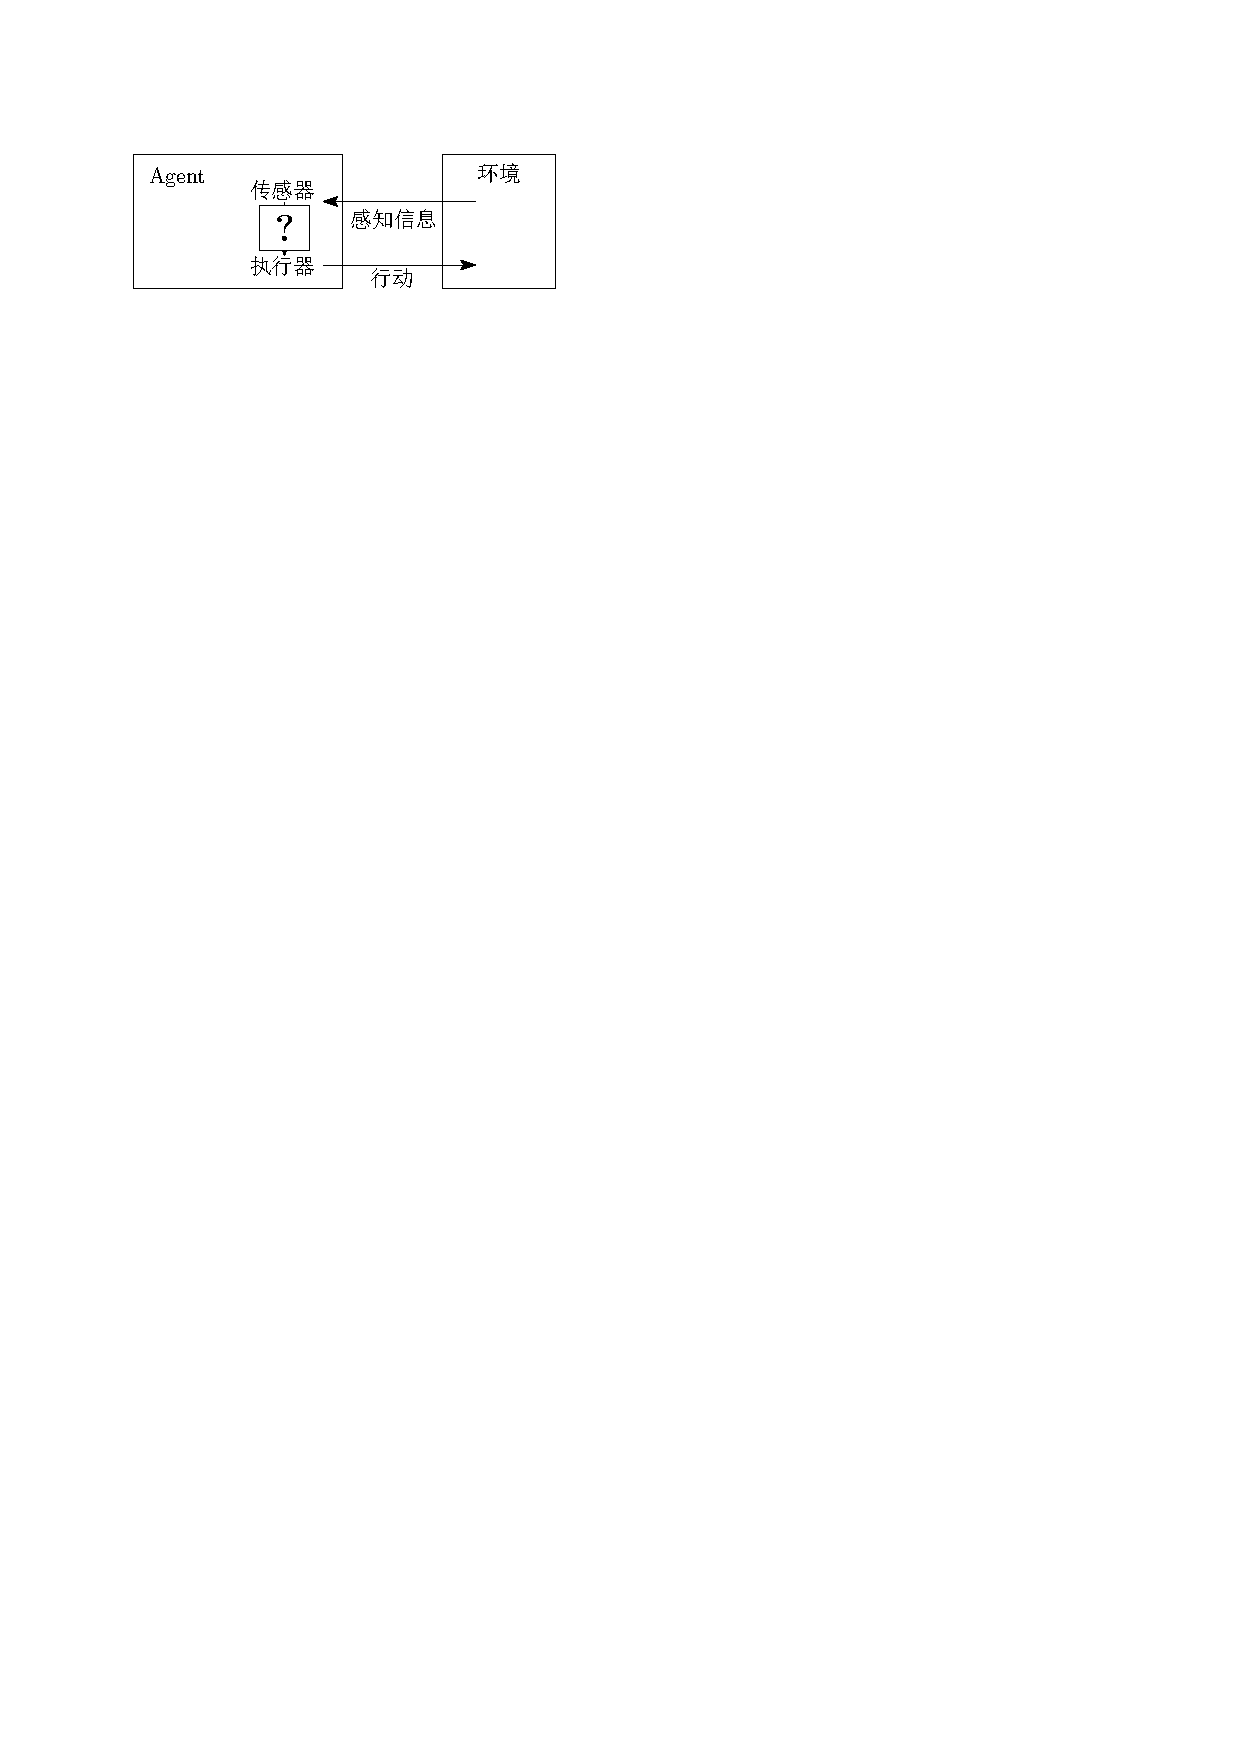
\includegraphics{image/Agent.pdf}
\end{figure}

\begin{itemize}
    \item Agent函数:将感知序列映射为行动:
    \[
        f:P^*\to A
    \]
    \item Agent程序:实现Agent函数,并在物理平台上运行
    \begin{center}
        \colorbox{main1}{Agent = 物理平台+\ Agent程序}
    \end{center}
\end{itemize}

Agent三个要素:
\begin{itemize}
    \item 感知环境能力
    \item 作用环境能力
    \item 感知信息与动作决策之间的映射机制
\end{itemize}

感知序列:
\begin{itemize}
    \item 有记忆
    \item 自身状态
    \item 之前的行为对当前决策与动作有影响
\end{itemize}

\begin{definition}[理性Agent]
    对每一个可能的感知信息,根据已知的感知序列提供的证据和Agent具有的先验知识,理性Agent应该选择能使其性能测度最大化的行动。
\end{definition}
\begin{definition}[性能测度]
    性能测度是对行动序列导致期望的环境变化的度量。
\end{definition}
性能测度对Agent的行为模型具有重要影响。

\begin{figure}[htbp]
    \centering
    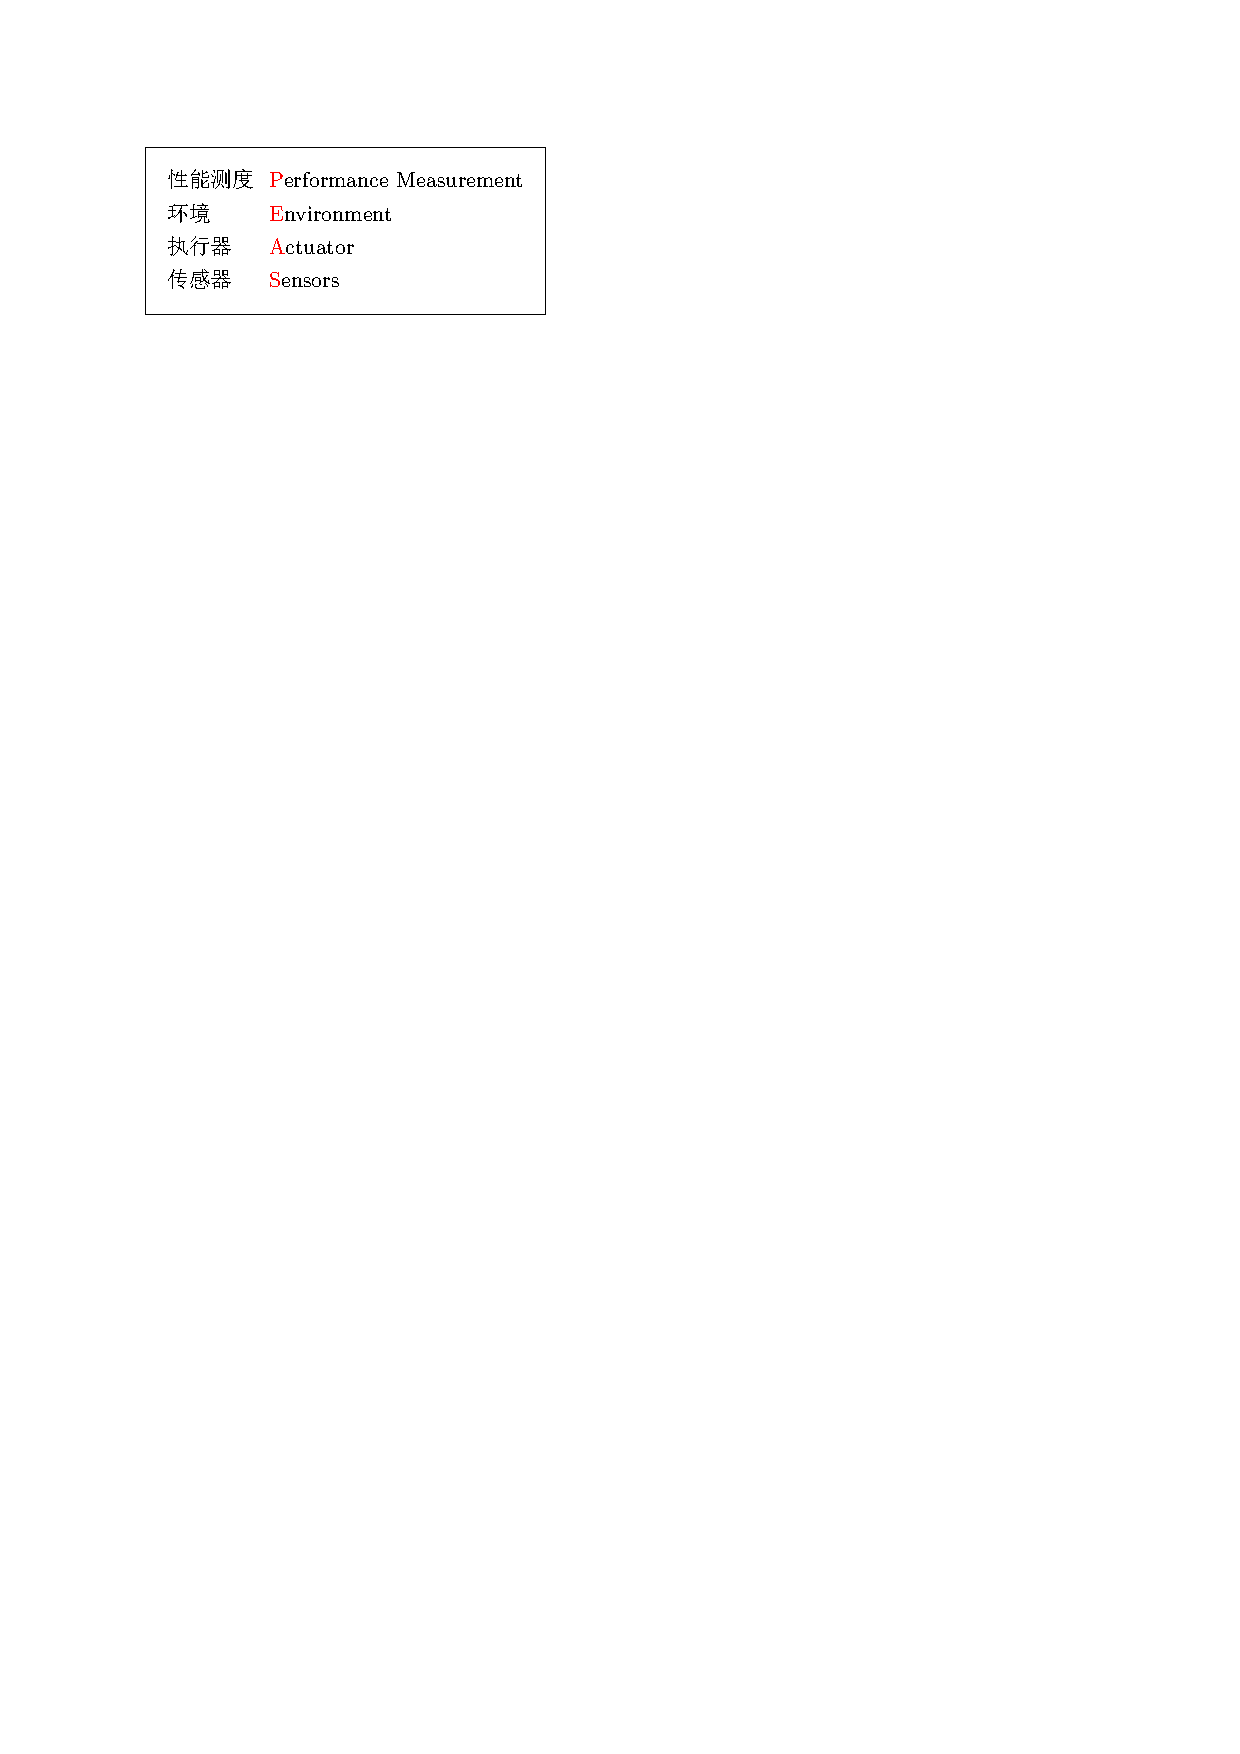
\includegraphics{image/PEAS.pdf}
\end{figure}

环境属性
\begin{itemize}
    \item 完全可观 vs 部分可观 (Fully observable vs. partially observable)
    \item 确定的 vs 随机的 (Deterministic vs. stochastic )
    \item 片段式vs 延续式(Episodic vs. sequential)
    \item 静态 vs 动态 (Dynamic vs. static )
    \item 离散 vs 连续 ( Discrete vs. continuous )
    \item 单Agent vs 多Agent ( Single agent vs. multi-agent )
    \item 已知 vs 未知 (Known vs. unknown)
\end{itemize}
% Table generated by Excel2LaTeX from sheet '环境属性'
\begin{table}[htbp]
    \centering
    \begin{tabular}{|c|ccc|}
      \hline
      任务环境 & 魔方Agnet & 吸尘器Agent & 无人侦察机 \bigstrut\\
      \hline
      完全可观 & 完全可观 & 部分可观 & 部分可观 \bigstrut[t]\\
      确定的 & 确定的 & 随机的 & 随机的 \\
      片段式 & 延续式 & 延续式 & 延续式 \\
      静态  & 静态  & 动态  & 动态 \\
      离散  & 离散  & 连续  & 连续 \\
      单Agent & 单   & 单   & 多 \\
      已知  & 已知  & 未知  & 未知 \bigstrut[b]\\
      \hline
    \end{tabular}%
\end{table}%

\begin{center}
    \colorbox{main1}{真实的环境是: 部分可观察、随机、延续、动态、连续、多Agent和未知。}
\end{center}
  
Agent类型:
\begin{figure}[htbp]
    \centering
    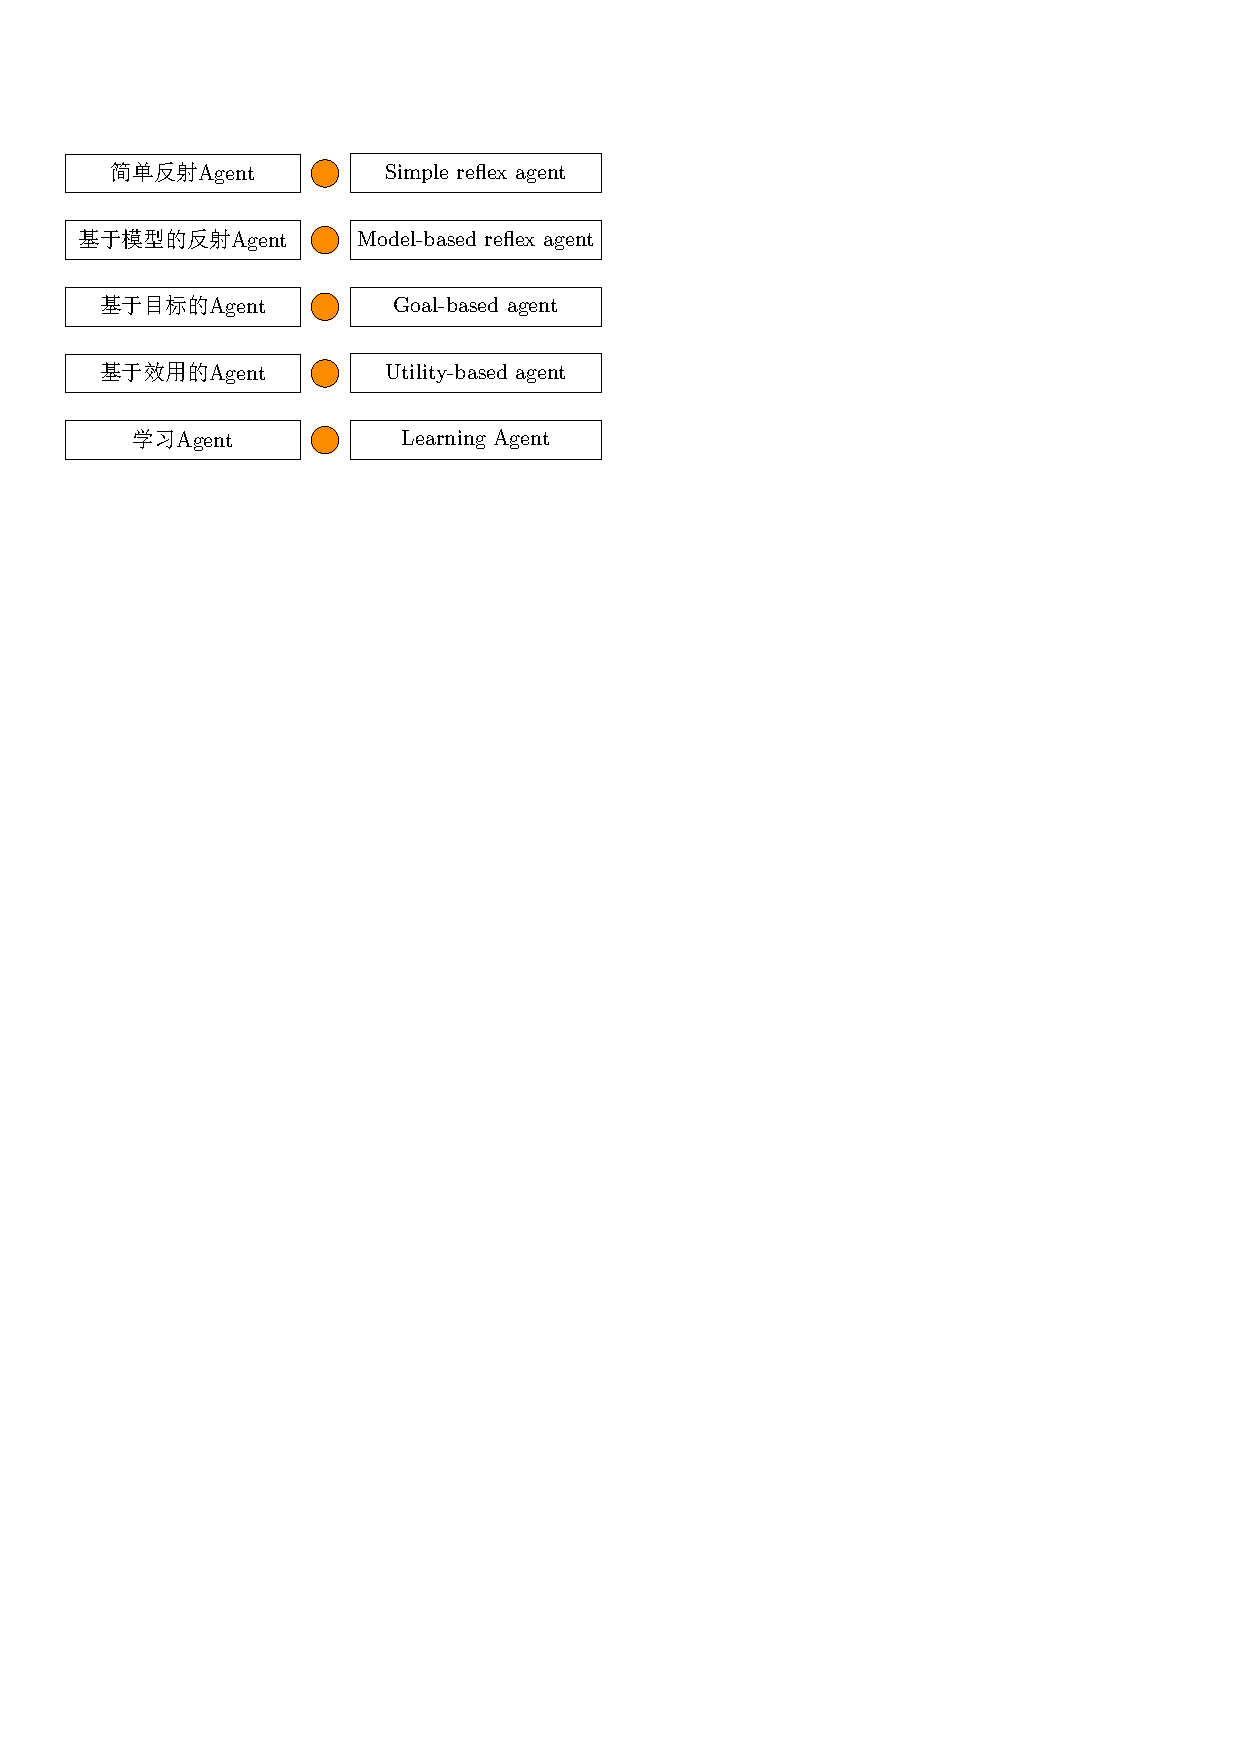
\includegraphics{image/Agent类型.pdf}
\end{figure}

\begin{definition}[简单反射Agent]
    简单反射Agent仅仅在当前感知的基础上动作忽略其余的感知历史。
\end{definition}
\begin{figure}[htbp]
    \centering
    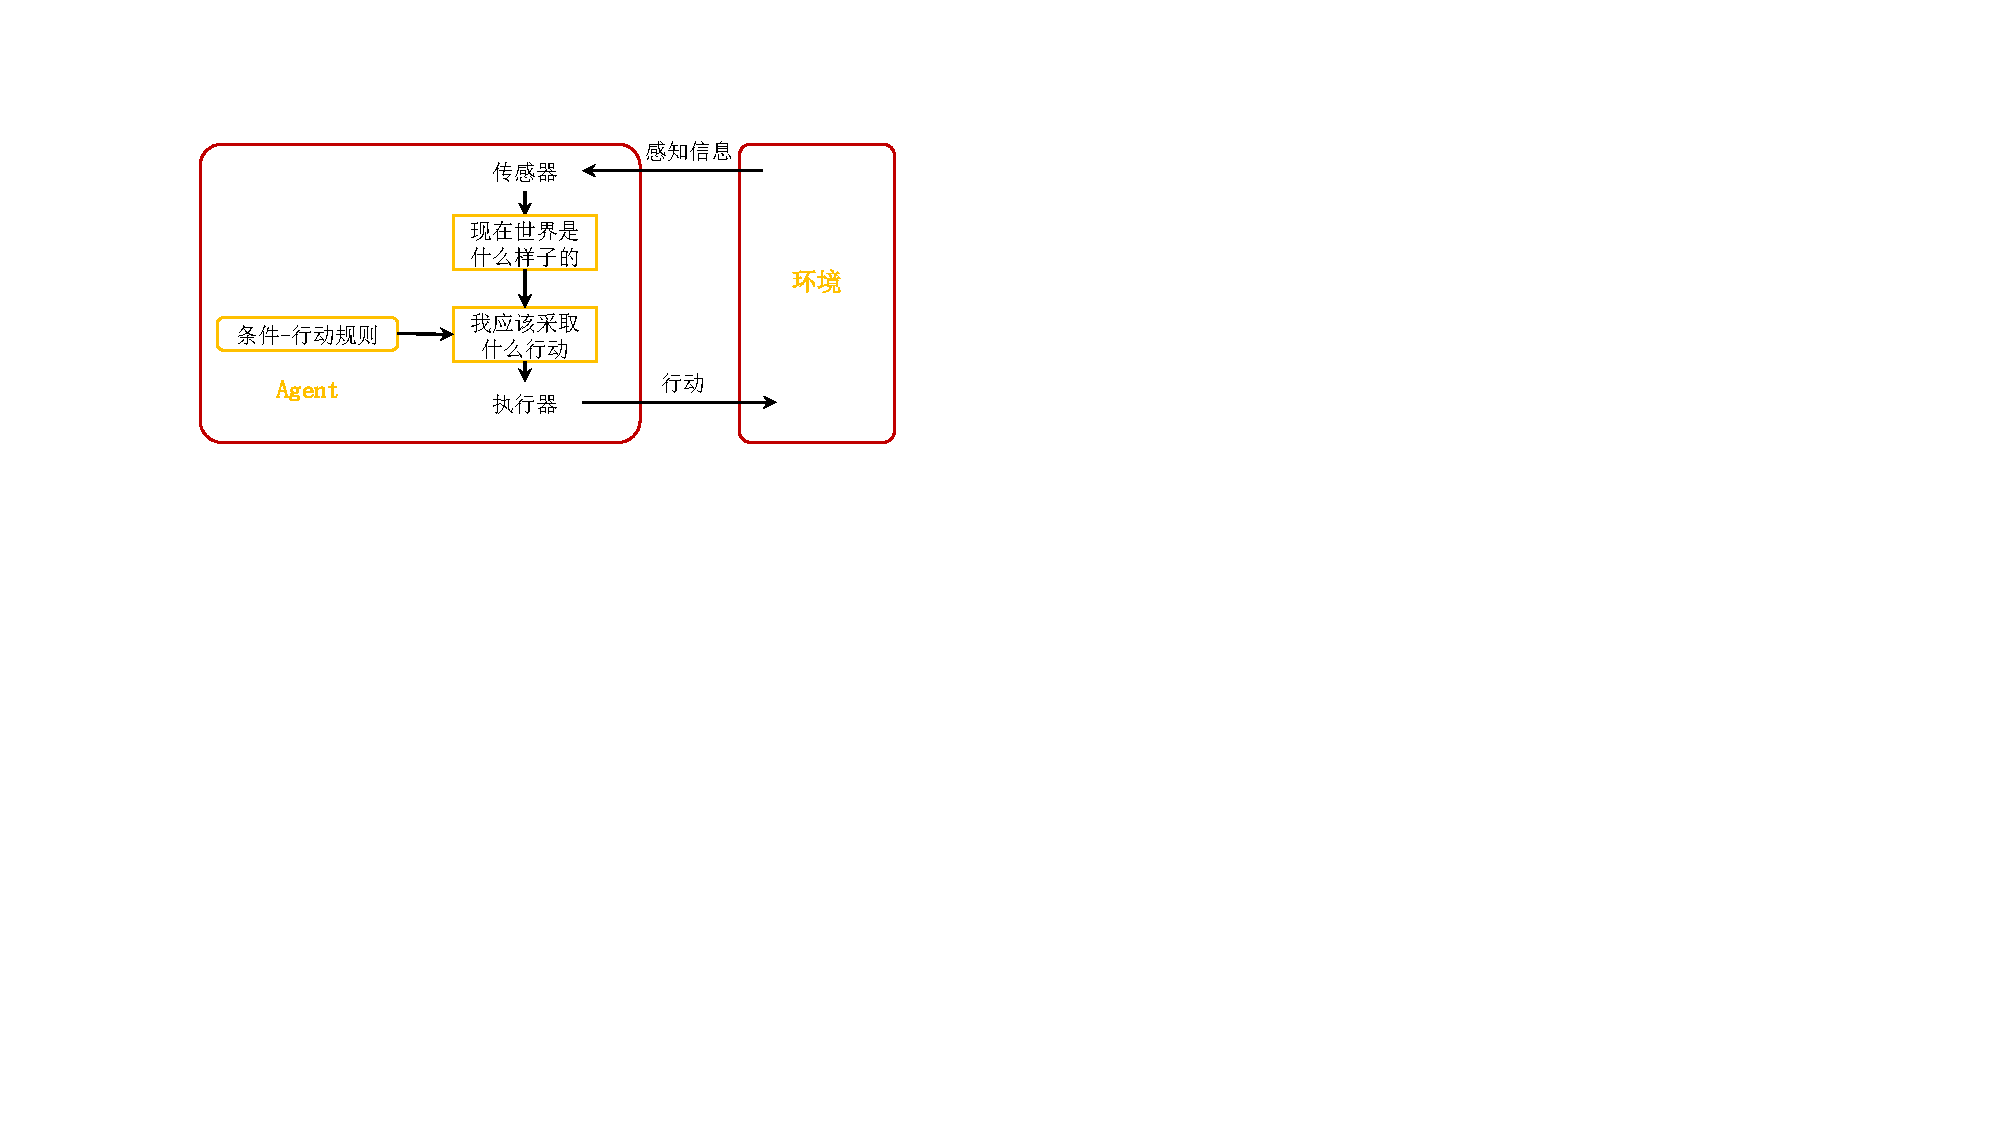
\includegraphics{image/简单反射Agent.pdf}
\end{figure}

\begin{definition}[基于模型的反射Agent]
    基于模型的反射Agent可以处理部分可观的环境。其当前状态存储在Agent内部,它描述不可见的环境的一部分。
\end{definition}
\begin{figure}[htbp]
    \centering
    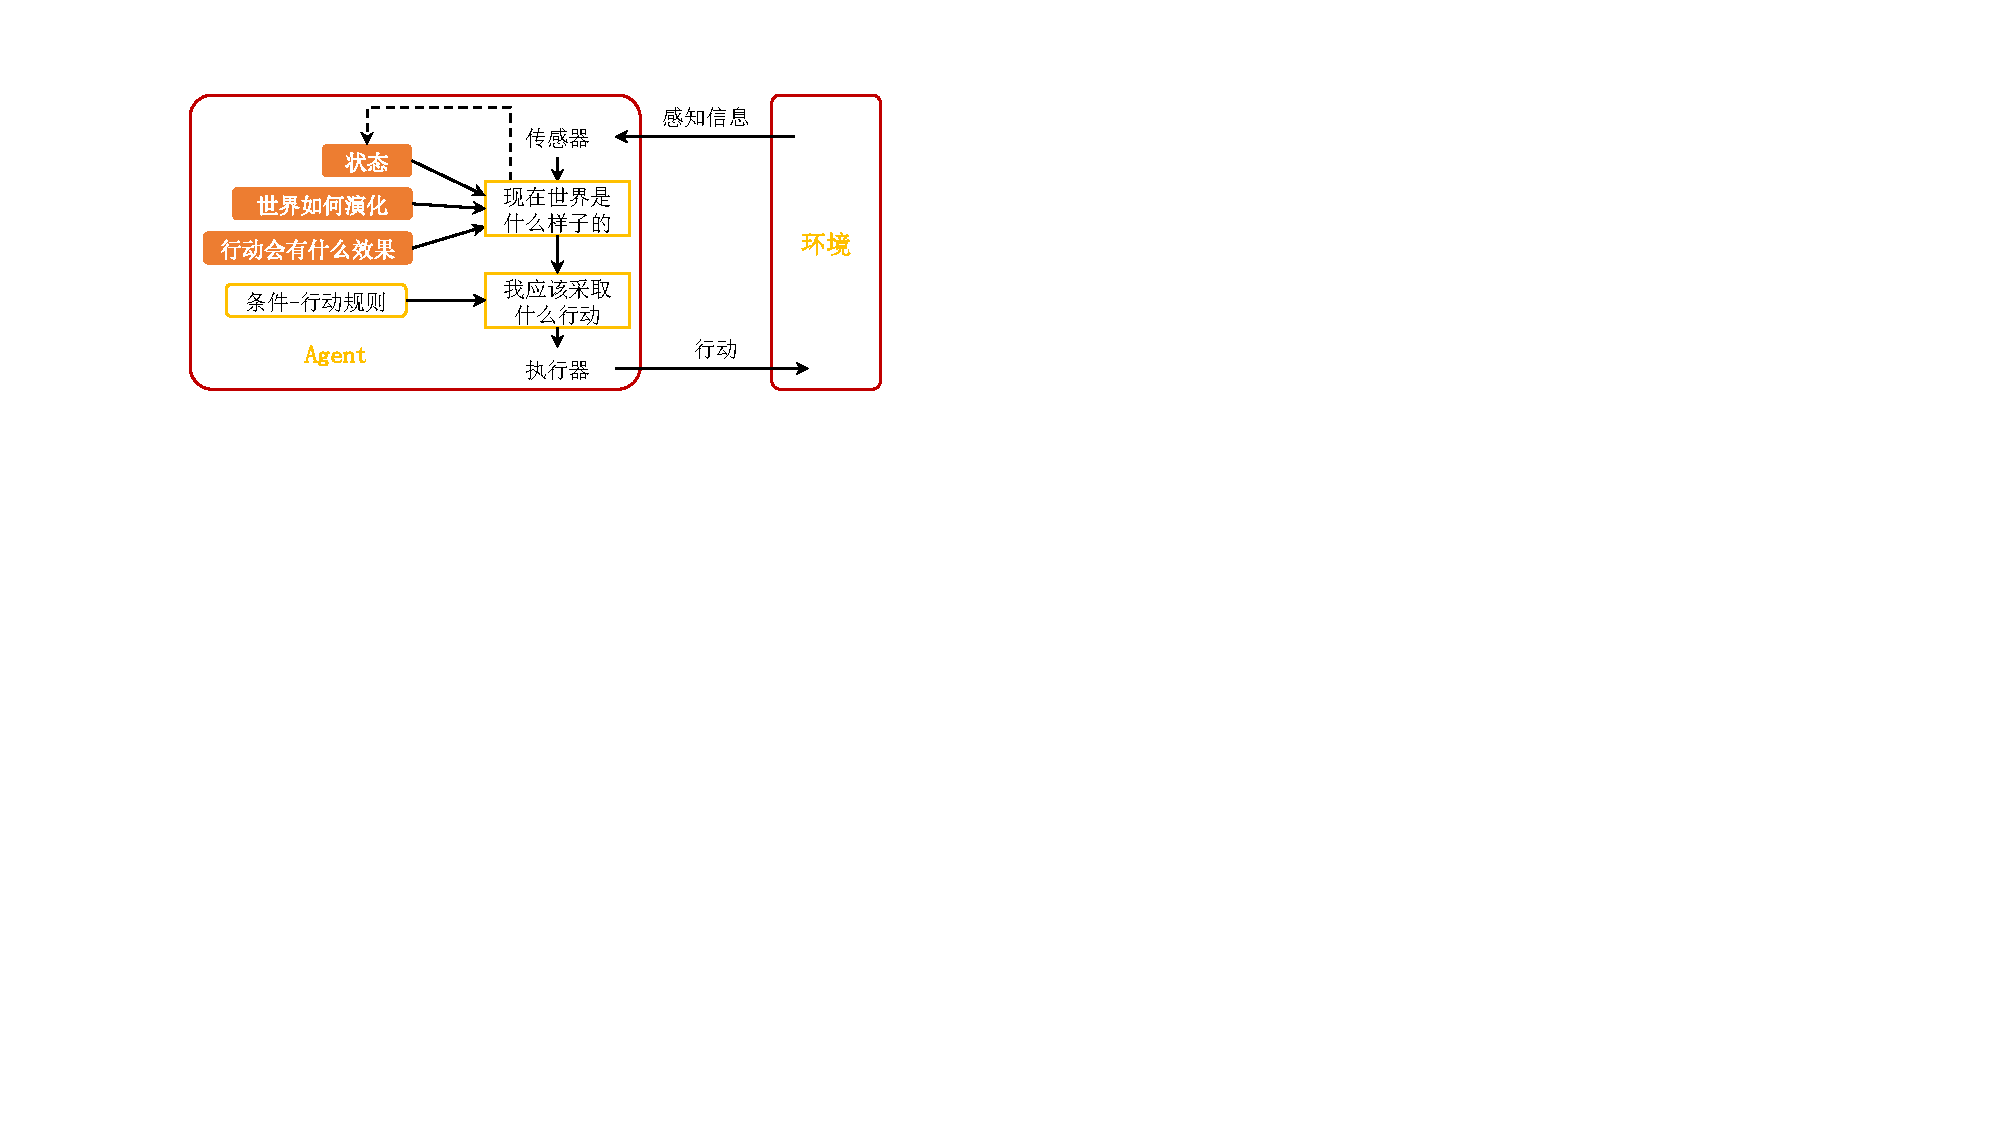
\includegraphics{image/基于模型的反射Agent.pdf}
\end{figure}

\begin{definition}[基于目标的Agent]
    利用“目标”信息,基于目标的Agent进一步扩展了基于模型的反射Agent的功能。  
\end{definition}
\begin{figure}[H]
    \centering
    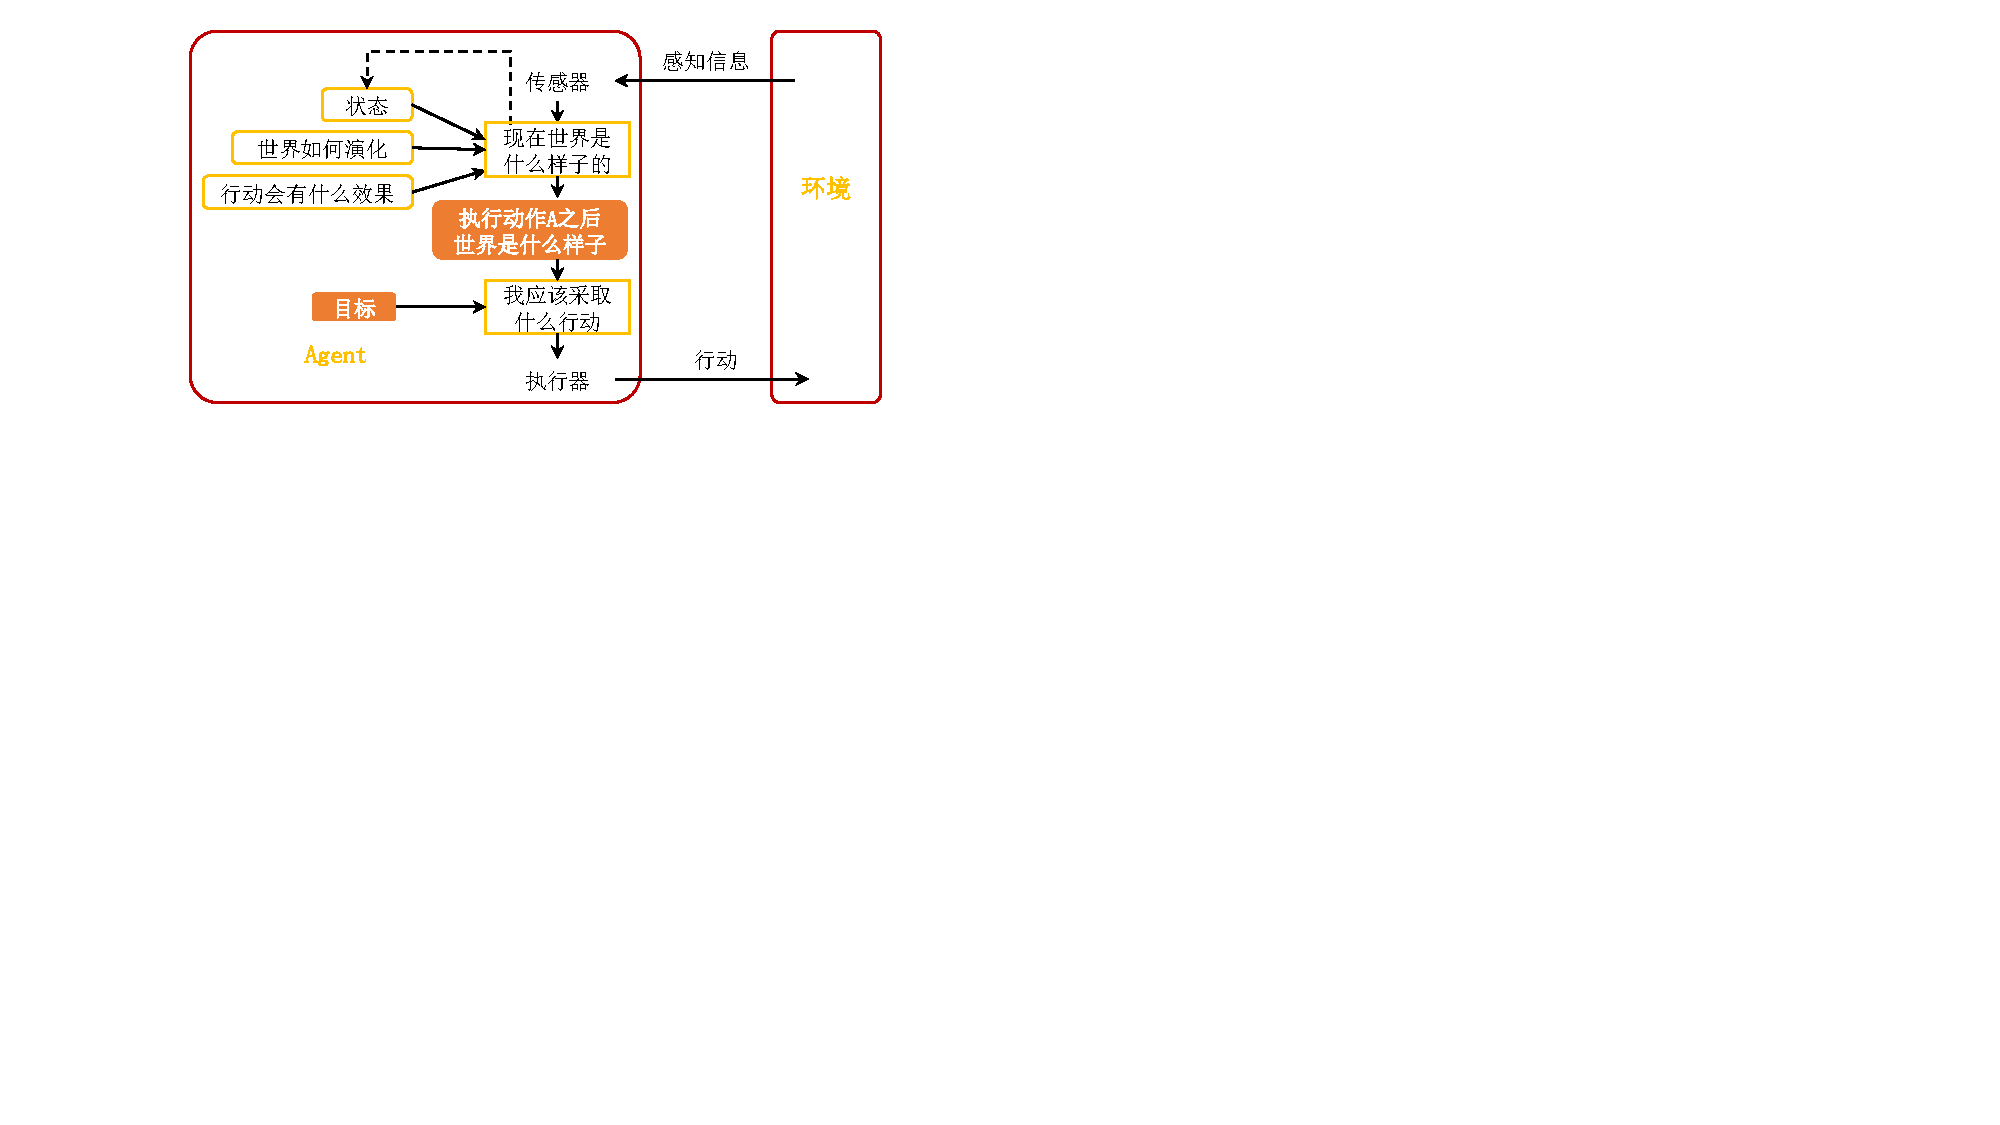
\includegraphics{image/基于目标的反射Agent.pdf}
\end{figure}

\begin{definition}[基于效用的Agent]
    使用效用函数得到对Agent的行动进行性能度量Agent选择最大效用的行动。
\end{definition}
\begin{figure}[H]
    \centering
    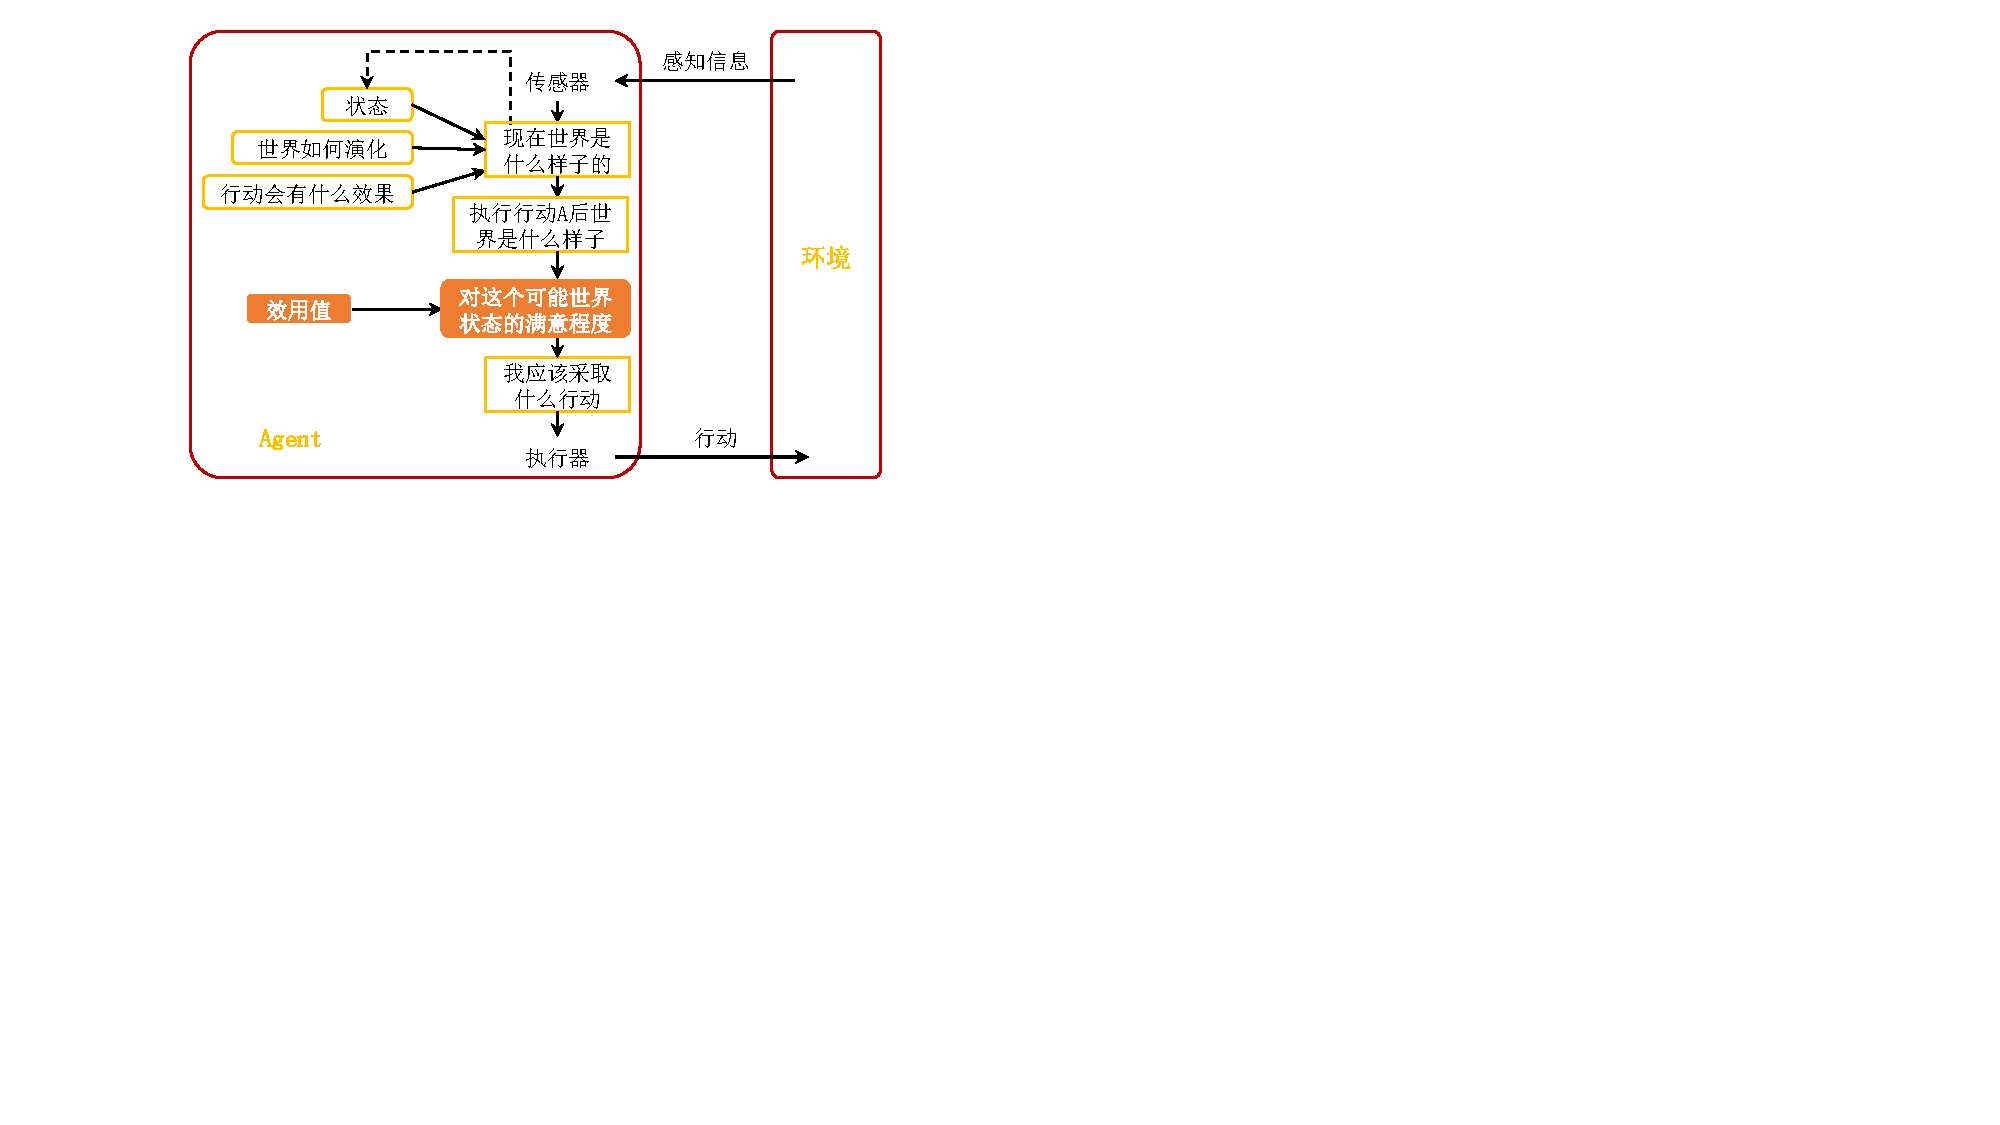
\includegraphics{image/基于效用的Agent.pdf}
\end{figure}

\begin{definition}[学习Agent]
    学习允许Agent在最初未知的环境中运行。与只具有最初知识相比,越来越胜任要执行的任务。 
\end{definition}
\begin{figure}[htbp]
    \centering
    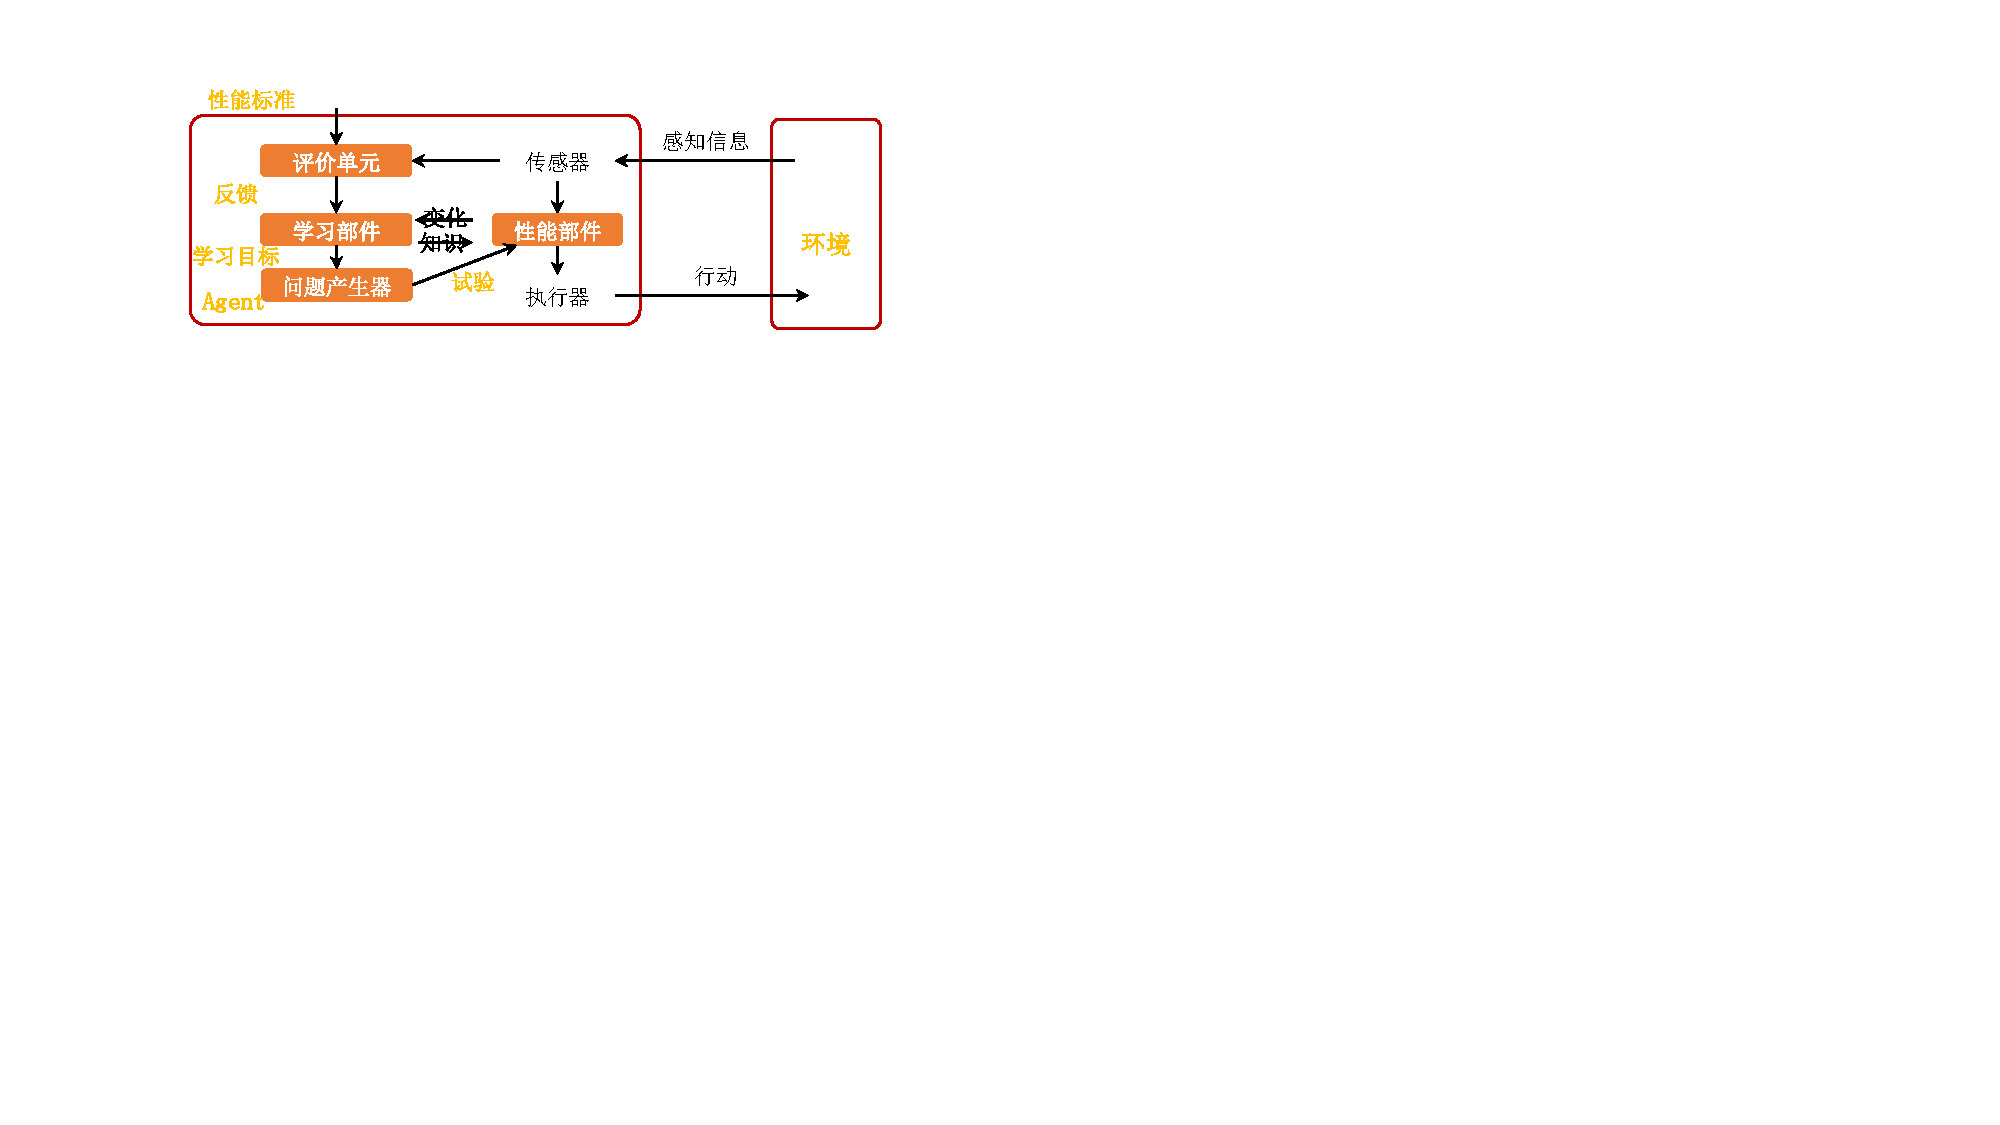
\includegraphics{image/学习Agent.pdf}
\end{figure}

表征环境状态的方式
\begin{itemize}
    \item 原子化
    
    每种状态都是内部结构未知的黑盒
    \item 要素化
    
    每种状态由固定的属性和值组成
    \item 结构化
    
    每个状态都包括对象,每个状态都具有与其他对象的属性和关系
\end{itemize}

  
  